% !Mode:: "TeX:UTF-8"
% !Mode:: "TeX:UTF-8"
\newcommand{\thepage}{} % to silence a hyperref warning about pdfpagelabels
\RequirePackage[]{silence}
\WarningsOff[hyperref]
\PassOptionsToPackage{log-declarations=false}{xparse}
%\RequirePackage[l2tabu, orthodox]{nag}
\RequirePackage{luatex85} % to make \pdf...= commands work with LuaTeX
\documentclass[aspectratio=169,t]{beamer}
\usepackage{ifthen}
\usepackage[T1]{fontenc}
\usepackage{iftex}
\ifLuaTeX
 \usepackage{fontspec}
 \setmainfont[Ligatures=TeX]{Source Sans Pro}
\else
 \usepackage[utf8]{inputenc}
\fi
\usepackage{german}
\usepackage{newunicodechar}
\newunicodechar{€}{\texteuro}
\newunicodechar{ß}{\ss}
\renewcommand{\SS}{\iffontchar\font"1E9E \symbol{"1E9E}\else SS\fi}
\usepackage{ellipsis}
\usepackage{microtype}
\usepackage{listings}
\usepackage{sourcecodepro}
\lstset{language=Python, basicstyle=\ttfamily}
\usepackage{amsfonts}
\usepackage{amssymb}
\usepackage{amsthm}
\usepackage{fancyhdr}
\usepackage{graphicx}

\newtheorem{proposition}[theorem]{Proposition}

\DeclareMathOperator*{\argmax}{argmax}
\DeclareMathOperator{\supp}{supp}
\newcommand{\E}{\ensuremath{\mathbb{E}}}
\newcommand{\V}{\ensuremath{\mathbb{V}}}

\setbeamercolor{emph}{fg=purple}
\renewcommand<>{\emph}[1]{%
  {\usebeamercolor[fg]{emph}\only#2{\itshape}#1}%
}



\hypersetup{draft=false,colorlinks=false,pdfpagemode=UseOutlines,plainpages=false,
            breaklinks=true,bookmarksnumbered=true,pdfborder=0 0 0,
            pdftitle={Data Science SoSe 2026 HHU},
            pdfauthor={Konrad Voelkel},
            pdfsubject={data science}}

%\documentclass[aspectratio=169,t]{beamer}
\usetheme{hhubeamer} % put the hhu-beamer-theme in /usr/share/texmf/tex/latex/beamer/themes/

% -------------------- Code listings config --------------------
% Define custom colors for syntax highlighting
\definecolor{codegreen}{rgb}{0,0.6,0}
\definecolor{codegray}{rgb}{0.5,0.5,0.5}
\definecolor{codepurple}{rgb}{0.58,0,0.82}
\definecolor{backcolour}{rgb}{0.96,0.96,0.94} % Very light gray/beige
% Configure the listings package
\lstset{
    language=Python,
    backgroundcolor=\color{backcolour},   
    commentstyle=\color{codegreen}\itshape,
    keywordstyle=\color{blue}\bfseries,
    numberstyle=\tiny\color{codegray},
    stringstyle=\color{codepurple},
    basicstyle=\ttfamily\footnotesize, % Use a monospaced font
    breakatwhitespace=false,         
    breaklines=true,      
             % Enable automatic line breaking
    captionpos=b,                      % Caption at the bottom
    keepspaces=true,                 
    numbers=left,                      % Line numbers on the left
    numbersep=10pt,                    % Distance of line numbers from the code
    showspaces=false,                
    showstringspaces=false,            % Don't show weird underscores in strings
    showtabs=false,                  
    tabsize=4,
    frame=single,                      % Add a subtle border around the code
    rulecolor=\color{black!20},        % Border color
  }

\event[]{}
\author[Sommersemester 2026]{Dr. Konrad Völkel, Sommersemester 2026}

%\title{Data Science, VL 1}
%\date{16.04.2026}


%%% Local Variables:
%%% mode: latex
%%% TeX-master: t
%%% End:


\title{Data Science, VL 10}
\subtitle{Multivariate Stochastik}
\date{26.05.2026}

\begin{document}

\begin{frame}
  \titlepage
\end{frame}

\begin{frame}
  \centering
  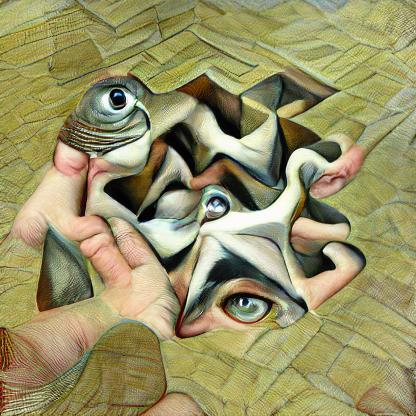
\includegraphics[height=0.8\textheight]{figures/escher.jpg} \\
  \textit{„Many dimensions at once, MC Escher“}
\end{frame}

\section{Gemeinsame Verteilungen und Marginalverteilungen}

\begin{frame}
  \frametitle{Gemeinsame Verteilungen}
  Zu zwei Zufallsvariablen $X \colon \Omega_1 \to \mathbb{R}$, $Y \colon \Omega_2 \to \mathbb{R}$ können wir das Produkt bilden:
  \[ X \times Y \colon \Omega_1 \times \Omega_2 \to \mathbb{R}^2, \quad (a,b) \mapsto (X(a), Y(b)) \]

  \pause\vspace{0.5cm}
  Sind die Definitionsbereiche identisch ($\Omega_1 = \Omega_2 = \Omega$), können wir das Produkt bilden:
  \[ X \times Y \colon \Omega^2 \to \mathbb{R}^2, \quad (a,b) \mapsto (X(a), Y(b)) \]
  und die Diagonalabbildung $\Delta \colon \Omega \to \Omega^2, a \mapsto (a,a)$ davorschalten, um die Zufallsvariable $(X,Y) \colon \Omega \to \mathbb{R}^2$ zu erhalten.
\end{frame}

\begin{frame}
  \frametitle{Marginalverteilungen}
  \begin{itemize}[<+->]
    \item Zu einer mehrdimensionalen Zufallsvariable $X \colon \Omega \to \mathbb{R}^n$ mit $X = (X_1, \dots, X_n)$ können wir die einzelnen $X_i \colon \Omega \to \mathbb{R}$ betrachten.
    \item Diese $X_i$ heißen \alert{Randverteilungen} oder \alert{Marginalverteilungen}.
    \item Allgemeiner ist auch ein Teilvektor wie $(X_1, X_3, X_9)$ eine Marginalverteilung.
    \item Wir können die Verteilung von $X_i$ berechnen:
    \[ P(X_i \in A) = P(X \in \pi_i^{-1}(A)) \]
    wobei $\pi_i \colon \mathbb{R}^n \to \mathbb{R}$ die Projektion auf die $i$-te Koordinate ist (denn $X_i = \pi_i \circ X$).
  \end{itemize}
\end{frame}

\begin{frame}
  \frametitle{Marginalverteilungen berechnen}
  Zu einer \textbf{diskreten} Zufallsvariable $(X,Y) \colon \Omega \to \mathbb{R}^2$ berechnet sich die Verteilung von $Y$ durch Ausintegrieren (Summieren) von $X$:
  \[ P(Y \in A) = \sum_{x \in X(\Omega)} P\big((X,Y) \in \{x\} \times A\big) \]
  \textit{(bzw. mit einem entsprechenden Integral im stetigen Fall)}

  \pause\vspace{0.5cm}
  Dabei haben wir $\pi_1^{-1}(A) = X(\Omega) \times A$ in disjunkte Teilmengen zerlegt.
\end{frame}

\begin{frame}
  \frametitle{Bedingte und gemeinsame Verteilung}
  Aus der Definition der bedingten Wahrscheinlichkeit $P(A \mid B) := \frac{P(A \cap B)}{P(B)}$ folgt die \alert{Summenregel}:
  \[ P((X,Y) = (x,y)) = P(X=x, Y=y) = P(Y=y \mid X=x) P(X=x) \]

  \pause\vspace{0.5cm}
  Für diskrete Zufallsvariablen schreiben wir das mit der Wahrscheinlichkeitsfunktion (PMF):
  \[ p_{X,Y}(x,y) = p_{Y|X}(y \mid x) p_X(x) \quad \iff \quad p_{Y|X}(y \mid x) := \frac{p_{X,Y}(x,y)}{p_X(x)} \]
  Dies ist für jedes konkrete $x$ die PMF der bedingten Verteilung. (Analog für stetige Zufallsvariablen mit der Dichtefunktion PDF).
\end{frame}

\begin{frame}
  \frametitle{Unabhängigkeit}
  Die Unabhängigkeit zweier Zufallsvariablen $X$ und $Y$ ist äquivalent dazu, dass sich die gemeinsame Dichte faktorisieren lässt:
  \[ p_{X,Y}(x,y) = p_Y(y) p_X(x) \]

  \pause\vspace{0.5cm}
  Dies ist wiederum äquivalent zu:
  \[ p_{Y|X}(y \mid x) = p_Y(y) \]
\end{frame}

\section{Bayessche Statistik}

\begin{frame}
  \centering
  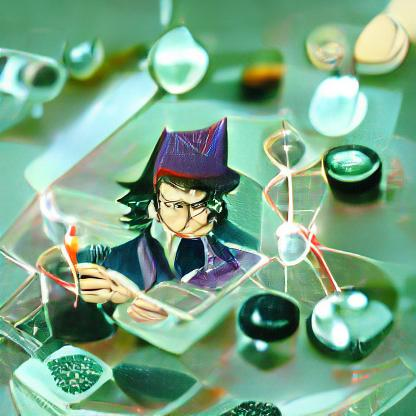
\includegraphics[height=0.8\textheight]{figures/magician.jpg} \\
  \textit{„Powerful magician looking at semiconductors“}
\end{frame}

\begin{frame}
  \frametitle{Der Satz von Bayes}
  Gegeben zwei Ereignisse $A, B \subseteq \Omega$. Aus dem Beweis $P(A \mid B) := \frac{P(A \cap B)}{P(B)}$ folgt:
  \[ P(A \mid B) = \frac{P(B \mid A) P(A)}{P(B)} \]

  \pause\vspace{0.5cm}
  Für Zufallsvariablen $X,Y \colon \Omega \to \mathbb{R}^n$:
  \[ P(Y=y \mid X=x) = \frac{P(X=x \mid Y=y) P(Y=y)}{P(X=x)} \]

  \pause\vspace{0.5cm}
  Häufige Anwendung:
  \begin{itemize}
    \item $X=x$ sind die \textbf{Daten $D$} (die sind bekannt).
    \item $Y=y$ ist unsere vorläufige \textbf{Hypothese $H$} (unser Modell).
  \end{itemize}
\end{frame}

\begin{frame}
  \frametitle{Bayessches Update}
  \vspace{-0.5cm}
  Gegeben eine Hypothese $H$ und Daten $D$:
  \[ \underbrace{P(H \mid D)}_{\text{Posterior}} = \frac{\overbrace{P(D \mid H)}^{\text{Likelihood}} \cdot \overbrace{P(H)}^{\text{Prior}}}{\underbrace{P(D)}_{\text{Evidenz}}} \]

  \pause\vspace{0.5cm}
  Die Wahrscheinlichkeit für die Hypothese unter Berücksichtigung der Daten zu berechnen, heißt \alert{Bayessches Update}.
  \begin{itemize}[<+->]
    \item \textbf{Prior:} $P(H)$
    \item \textbf{Likelihood:} $P(D \mid H)$, „how likely is the data, if the hypothesis were true?“
    \item \textbf{Evidenz:} $P(D)$
    \item \textbf{Posterior:} $P(H \mid D)$
  \end{itemize}
\end{frame}

\begin{frame}
  \frametitle{Die Likelihood in der Praxis}
  Denken wir an die 3 Verteilungen: Datenerzeugung $X \to$ Daten $D \to$ Modell $Y$.

      \vspace{0.3cm}
  Die Likelihood $P(X=D \mid Y=D)$ gibt an, wie wahrscheinlich es ist, die Daten $D$ zu sehen, wenn man $Y$ zur Erzeugung der Daten nimmt.

  \pause\vspace{0.5cm}
  \textbf{Beispiel:}
  Angenommen, wir rechnen fest mit einer Normalverteilung $\mathcal{N}(\mu, \sigma^2)$ mit Dichte $p_{\mu,\sigma}$.
  Hypothese $H$: $\mu=0, \sigma=2$.

      \vspace{0.3cm}
  Dann ist $P(X=D \mid H)$ die Wahrscheinlichkeit für ein Sample $D$ unter $X \sim \mathcal{N}(0, 2^2)$.
  Die Likelihood(-Dichte) ist das Produkt: $\prod_{x \in D} p_{\mu,\sigma}(x)$.
\end{frame}

\section{Kovarianz und Varianz}

\begin{frame}
  \frametitle{Kovarianz}
  \begin{definition}
    Gegeben eine bivariate Zufallsvariable $(X,Y) \colon \Omega \to \mathbb{R}^2$. Die \alert{Kovarianz} ist definiert als:
    \[ Cov(X,Y) := \E\big((X - \E X)(Y - \E Y)\big) \]
  \end{definition}

  \pause\vspace{0.3cm}
  Also auch: $\V(X) = Cov(X,X)$.

  \pause\vspace{0.5cm}
  Die Kovarianz hat die gleiche Krankheit wie die Varianz: sie ist skalenabhängig. Zur Heilung normiert man mit den Standardabweichungen.
\end{frame}

\begin{frame}
  \frametitle{Korrelationskoeffizient}
  \begin{definition}
    (Pearsons) \alert{Korrelationskoeffizient} $\rho(X,Y)$ ist definiert als:
    \[ \rho(X,Y) := \frac{Cov(X,Y)}{\sigma(X)\sigma(Y)} \]
  \end{definition}

  \pause\vspace{0.3cm}
  \begin{itemize}[<+->]
    \item Es ist klar: $\rho(X,Y) = 0 \iff Cov(X,Y) = 0$.
    \item $X$ und $Y$ sind \alert{positiv korreliert}, wenn $\rho(X,Y) > 0$.
    \item $X$ und $Y$ sind \alert{unkorreliert}, wenn $\rho(X,Y) = 0$.
  \end{itemize}
\end{frame}

\begin{frame}[fragile]
  \frametitle{Visualisierung einer bivariaten Verteilung}
  \vspace{-1cm}
\begin{lstlisting}[language=Python]
import numpy as np
import scipy.stats as st
import matplotlib.pyplot as plt

origin = [0,0] #
Sigma = [[1,2],[0,1]] #
Z = st.multivariate_normal(origin, cov=Sigma) #
sample = Z.rvs(10000) #
x, y = sample[:,0], sample[:,1] #

fig, axs = plt.subplots(2, 2, figsize=(12,12)) #
axs[0,1].scatter(x, y, alpha=0.05) #
axs[1,1].hist(x, bins=100) #
axs[0,0].hist(y, bins=100, orientation="horizontal") #
plt.show() #
\end{lstlisting}
\end{frame}

\begin{frame}
  \vspace{-1cm}
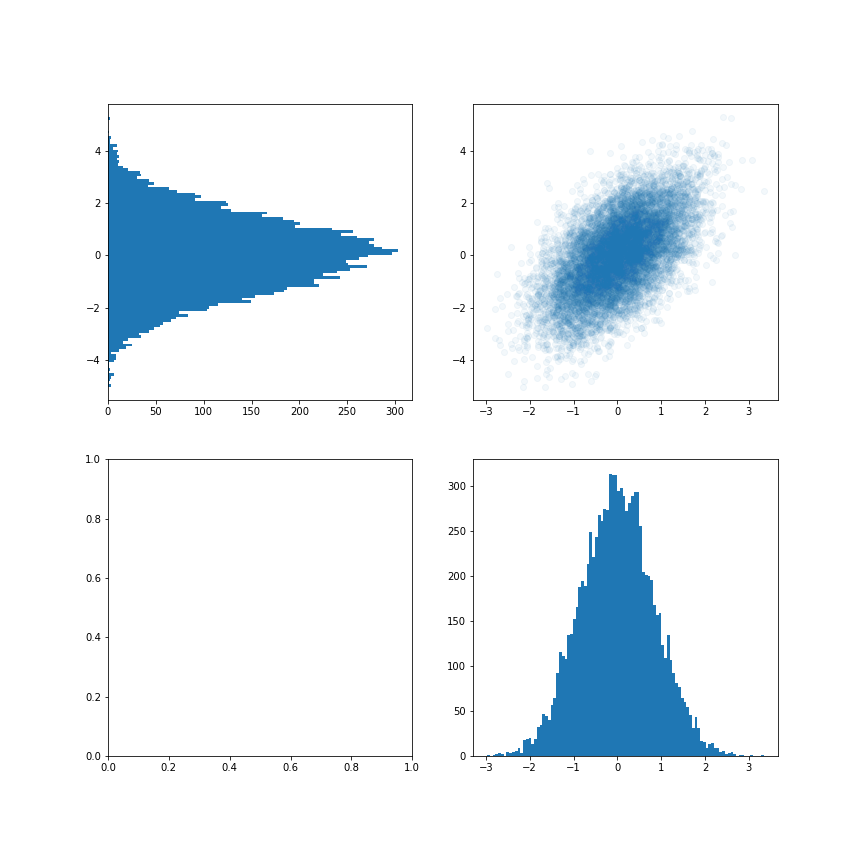
\includegraphics[height=1.1\textheight]{figures/normalmarginal.png}
\end{frame}

\begin{frame}
  \frametitle{Kovarianz: Der Datasaurus}
  \textit{Matejka, Fitzmaurice: Same Stats, Different Graphs (2017)}

  \centering
  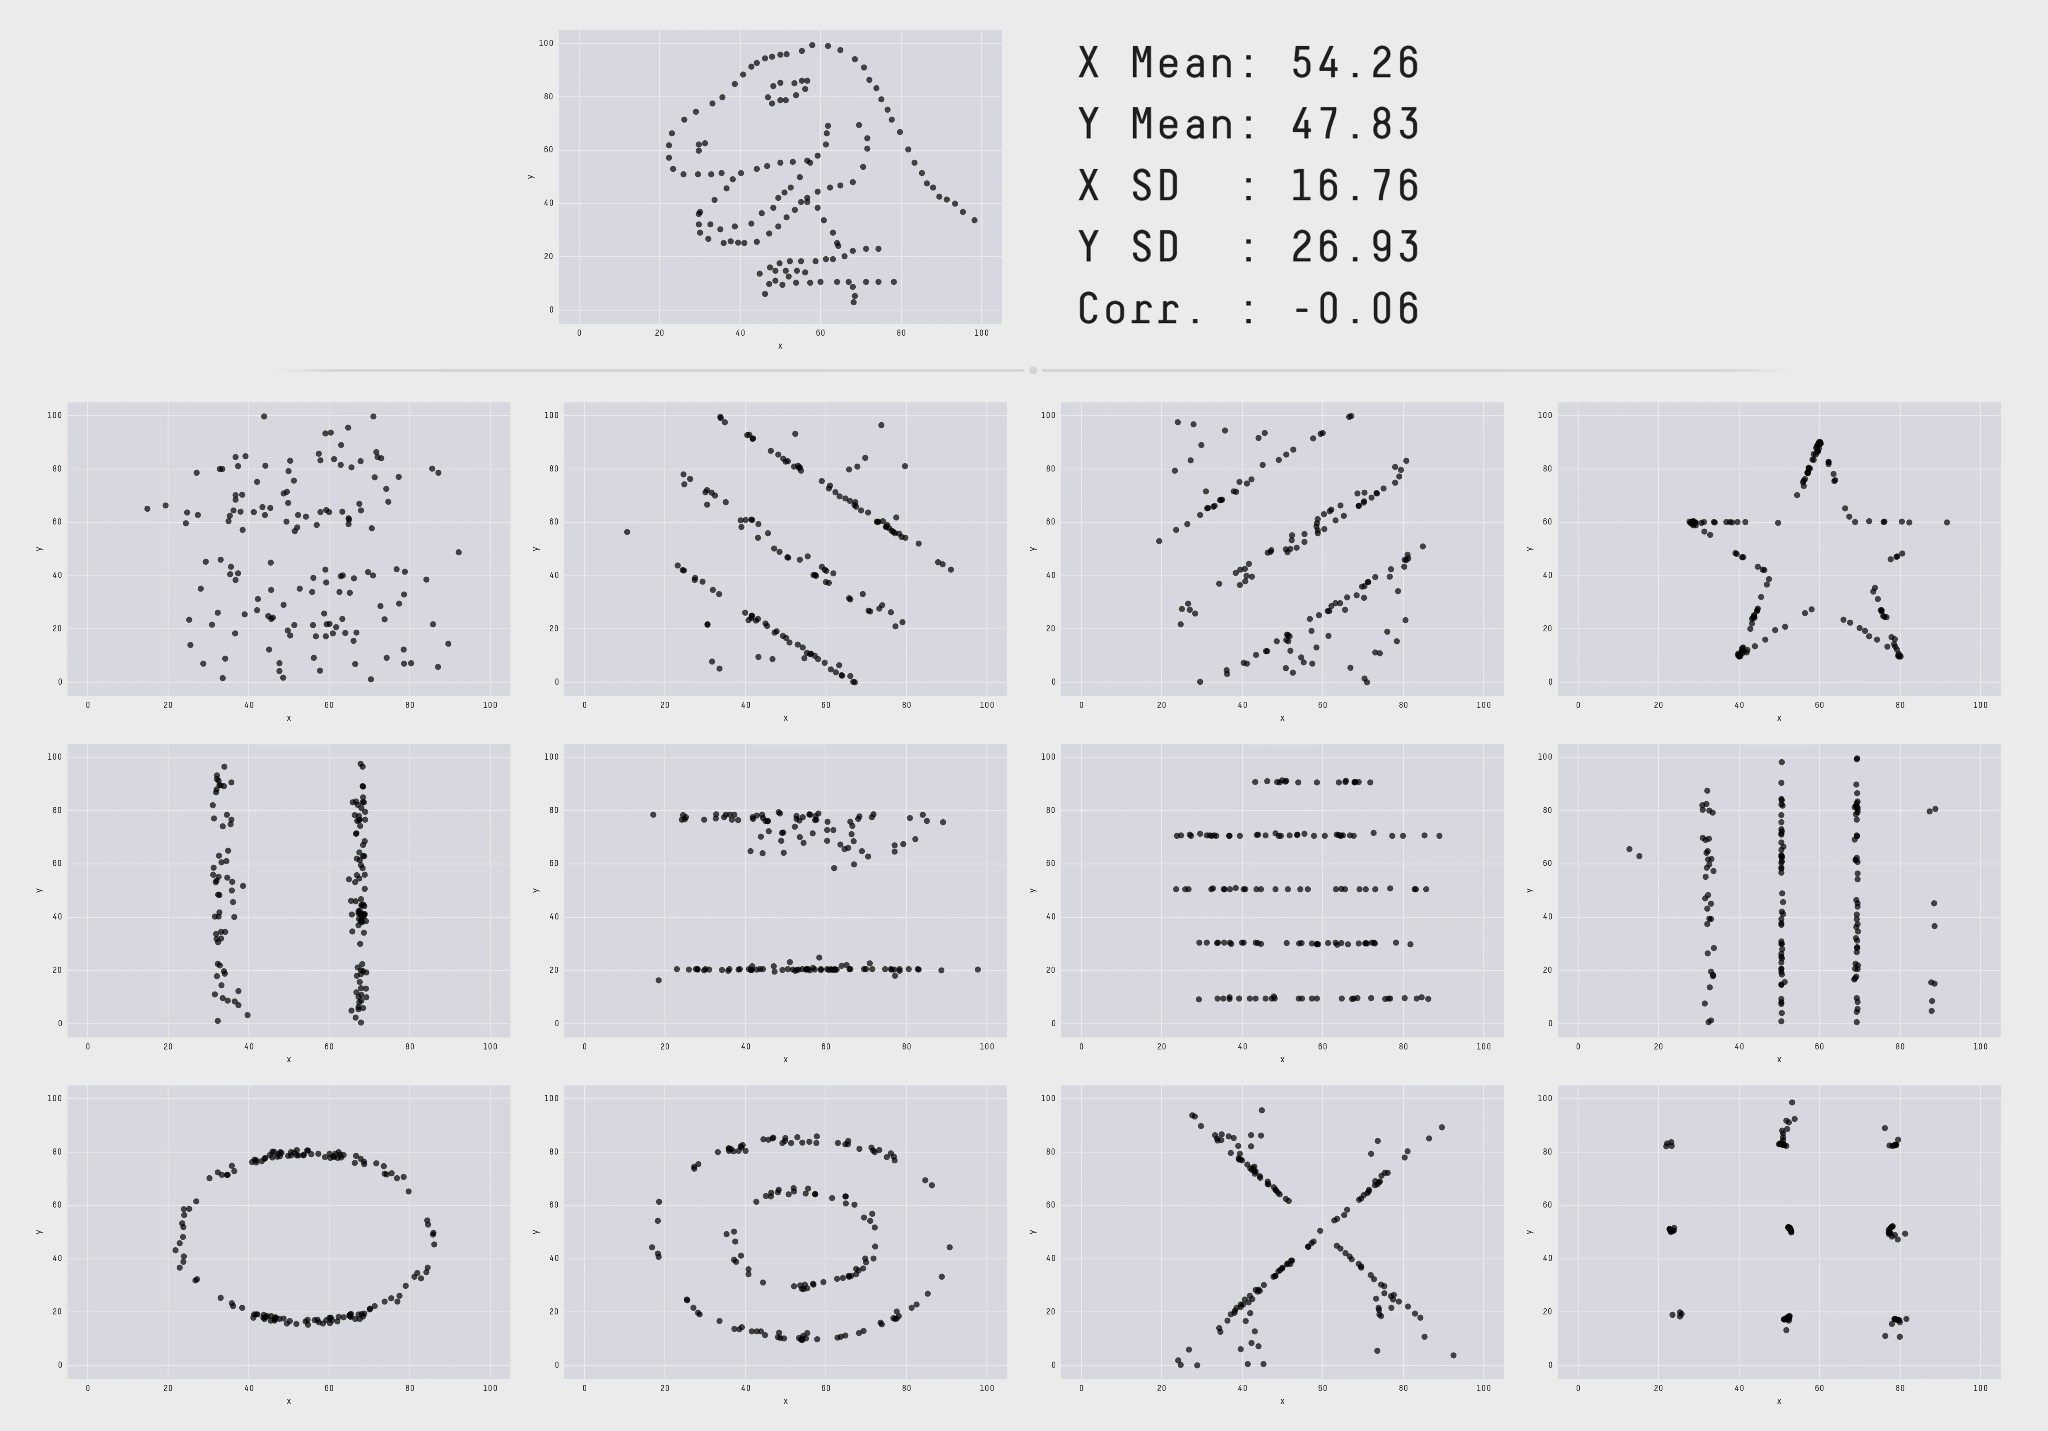
\includegraphics[width=0.8\textwidth]{figures/datasaurus.png}

      \vspace{0.3cm}
  All diese gezeigten Verteilungen haben den \alert{gleichen Korrelationskoeffizienten}!
\end{frame}

\begin{frame}
  \frametitle{Eigenschaften der Kovarianz}
  Die Kovarianz ist symmetrisch und bilinear:
  \begin{itemize}[<+->]
    \item \textbf{Symmetrie:} $Cov(X,Y) = Cov(Y,X)$
    \item \textbf{Bilinearität:} Für $a,b \in \mathbb{R}$ ist:
    \[ Cov(aX + bY, Z) = a \cdot Cov(X,Z) + b \cdot Cov(Y,Z) \]
    \item \textbf{Positiv definit:} $Cov(X,X) \geq 0$ und $Cov(X,X) = 0$ nur für konstantes $X$.
  \end{itemize}
\end{frame}

\begin{frame}[separator]
  \frametitle{Danke für Ihre Aufmerksamkeit.}
\end{frame}

\end{document}

%%% Local Variables:
%%% mode: latex
%%% TeX-master: t
%%% End:
